%% This is file `DEMO-TUDaBeamer.tex' version 3.10 (2021/02/22),
%% it is part of
%% TUDa-CI -- Corporate Design for TU Darmstadt
%% ----------------------------------------------------------------------------
%%
%%  Copyright (C) 2018--2021 by Marei Peischl <marei@peitex.de>
%%
%% ============================================================================
%% This work may be distributed and/or modified under the
%% conditions of the LaTeX Project Public License, either version 1.3c
%% of this license or (at your option) any later version.
%% The latest version of this license is in
%% http://www.latex-project.org/lppl.txt
%% and version 1.3c or later is part of all distributions of LaTeX
%% version 2008/05/04 or later.
%%
%% This work has the LPPL maintenance status `maintained'.
%%
%% The Current Maintainers of this work are
%%   Marei Peischl <tuda-ci@peitex.de>
%%   Markus Lazanowski <latex@ce.tu-darmstadt.de>
%%
%% The development respository can be found at
%% https://github.com/tudace/tuda_latex_templates
%% Please use the issue tracker for feedback!
%%
%% If you need a compiled version of this document, have a look at
%% http://mirror.ctan.org/macros/latex/contrib/tuda-ci/doc
%% or at the documentation directory of this package (if installed)
%% <path to your LaTeX distribution>/doc/latex/tuda-ci
%% ============================================================================
%%
% !TeX program = lualatex
%%

%% This is file `DEMO-TUDaBeamer.tex' version 3.10 (2021/02/22),
%% it is part of
%% TUDa-CI -- Corporate Design for TU Darmstadt
%% ----------------------------------------------------------------------------
%%
%%  Copyright (C) 2018--2021 by Marei Peischl <marei@peitex.de>
%%
%% ============================================================================
%% This work may be distributed and/or modified under the
%% conditions of the LaTeX Project Public License, either version 1.3c
%% of this license or (at your option) any later version.
%% The latest version of this license is in
%% http://www.latex-project.org/lppl.txt
%% and version 1.3c or later is part of all distributions of LaTeX
%% version 2008/05/04 or later.
%%
%% This work has the LPPL maintenance status `maintained'.
%%
%% The Current Maintainers of this work are
%%   Marei Peischl <tuda-ci@peitex.de>
%%   Markus Lazanowski <latex@ce.tu-darmstadt.de>
%%
%% The development respository can be found at
%% https://github.com/tudace/tuda_latex_templates
%% Please use the issue tracker for feedback!
%%
%% If you need a compiled version of this document, have a look at
%% http://mirror.ctan.org/macros/latex/contrib/tuda-ci
%% ============================================================================
%%
% !TeX program = lualatex
%%

\documentclass[
	ngerman,%globale Übergabe der Hauptsprache
	aspectratio=169,%Beamer eigene Option zum Umschalten des Formates
	color={accentcolor=2d},
	logo=true,%Kein Logo auf Folgeseiten
	colorframetitle=true,%Akzentfarbe auch im Frametitle
%	logofile=example-image, %Falls die Logo Dateien nicht vorliegen
	]{tudabeamer}
\usepackage[main=ngerman]{babel}
\usepackage{iftex}
\ifPDFTeX
\usepackage[utf8]{inputenc}%kompatibilität mit TeX Versionen vor April 2018
\fi


%Makros für Formatierungen der Doku
%Im Allgemeinen nicht notwendig!
\let\code\texttt

\title{A Workflow for Increasing the Quality of Scientific Software}
\subtitle{SIAM Conference on Computational Science and Engineering 2021-03-01}
\author[T. Mari\'c, JP. Lehr, I. Pappagianidis, B. Lambie, D. Bothe, C. Bischof]{Tomislav Mari\'c}
\department{TU Darmstadt, Germany}
\institute{CRC 1194 : Z-INF}


%Fremdlogo
%Logo Macro mit Sternchen skaliert automatisch, sodass das Logo in die Fußzeile passt
\logo*{
\includegraphics{./crc-logo}}

% Da das Bild frei wählbar nach Breite und/oder Höhe skaliert werden kann, werden \width/\height entsprechend gesetzt. So kann die Fläche optimal gefüllt werden.
%Sternchenversion skaliert automatisch und beschneidet das Bild, um die Fläche zu füllen.
%\titlegraphic*{\includegraphics{example-image}}
\titlegraphic{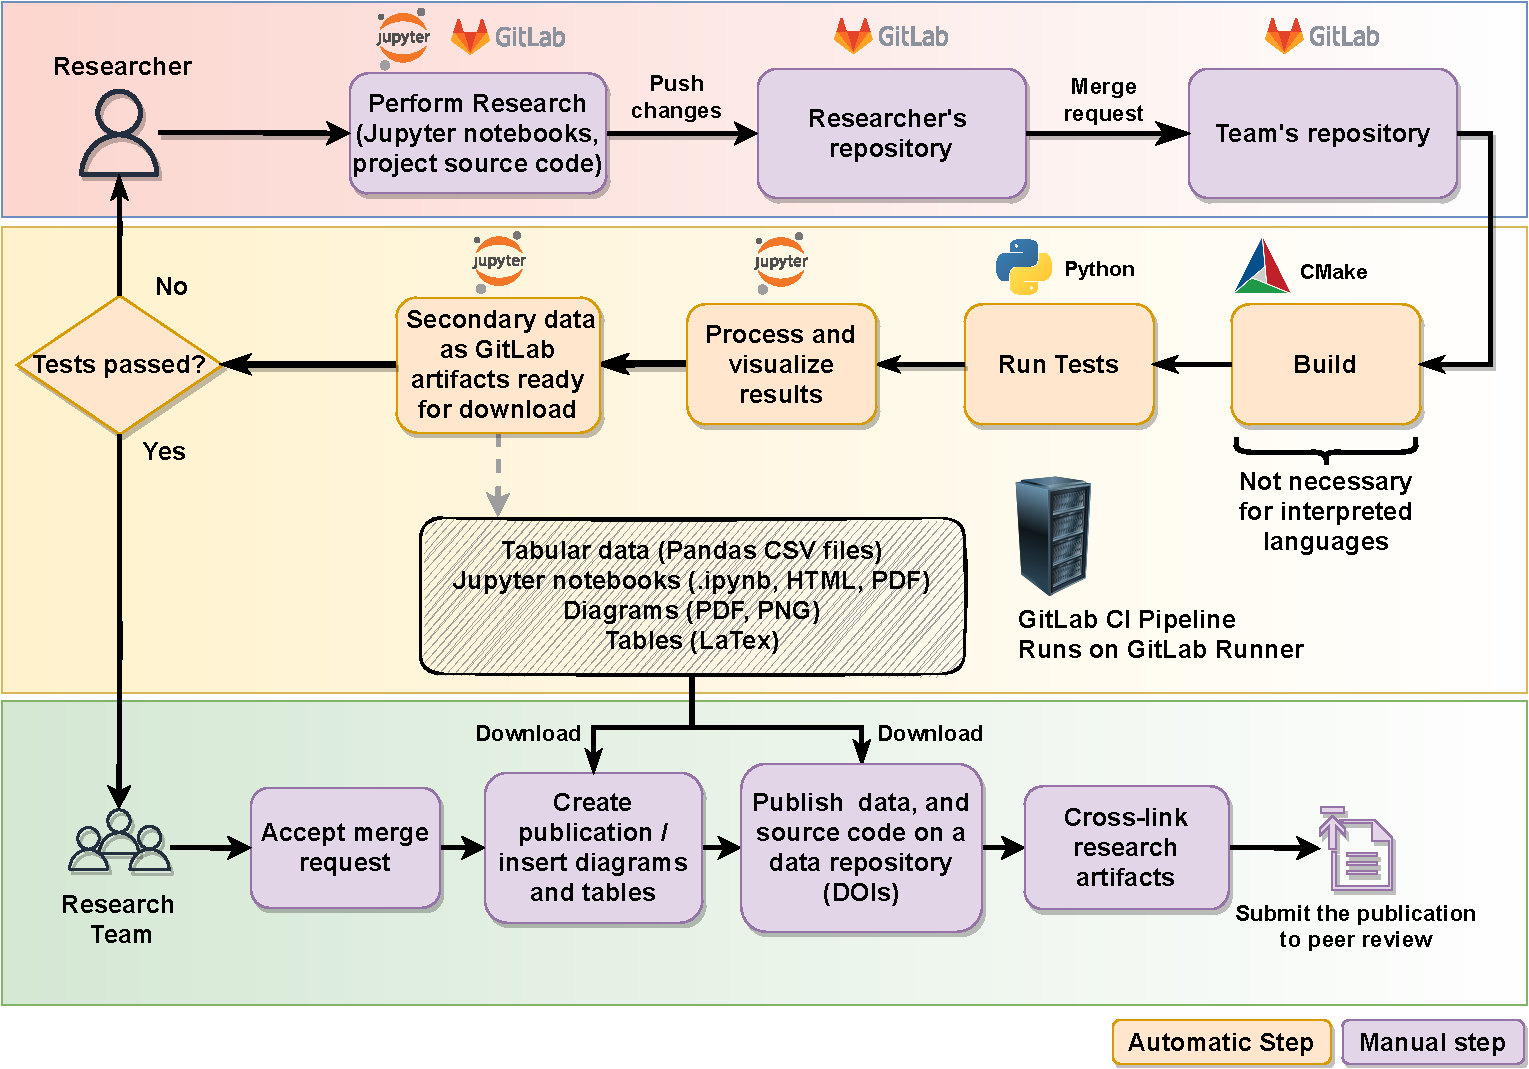
\includegraphics[scale=0.47]{figures/ZINF-CI-diagram.pdf}}
\date{2021-03-01}

\begin{document}

\maketitle

\begin{frame}{CSE software at university research groups}
	\framesubtitle{Boundary and initial conditions}
	
	\vfill
	\begin{itemize}
		\item Publish or perish culture: software is not a priority, publications are.
		\item Dedicated resources for increasing software quality are usually not available.
		\item Ph.D. students rotate every ~4-5 years, postdocs every 1-2 years. 
			\begin{itemize}
				\item Little or no overlap between successors and predecessors. 
			\end{itemize}
		\item Large-scale software design is not a necessary part of the curriculum. 
			\begin{itemize}
				\item Different backgrounds: (Applied) Mathematics, Mechanical Engineering, Physics, CSE.
			\end{itemize}
		\item Real-world example: onboarding students into \href{https://www.openfoam.com/documentation/guides/latest/api/classes.html}{\beamergotobutton{OpenFOAM}} module development.
	\end{itemize}
\end{frame}

\begin{frame}{CSE software at university research groups}
	\framesubtitle{Divergence}
	
	\vfill
	\begin{itemize}
		\item Not being able to continue development from an earlier state.
		\item Reproducing results from a publication is not possible.  
			\begin{itemize}
				\item Data, source code and publication are not archived and cross-linked. 
				\item The version used to generate the data is not documented. 
			\end{itemize}
		\item Not being able to re-use a model from a publication. 
			\begin{itemize}
				\item The model is not implemented in a modular way.
				\item Version integration was not done.
				\item Non-granular commits were used. 
			\end{itemize}
		\item Having no overview of the impact of a contribution on the rest of the module.
	\end{itemize}

	\medskip

\end{frame}

\begin{frame}{A workflow for increasing the quality of (academic) CSE software} 

	\vfill
	The academic CSE software quality workflow: 
	\begin{enumerate}
		\item Track the issues in a Kanban board.
		\item Use a pragmatic version-control branching model. 
		\item Apply Test-Driven Development (TDD) to CSE results.  
		\item Enable Continuous Integration with an emphasis on result visualization. 
		\item Cross-link software, result data, and report/article when reaching a milestone.
			\begin{itemize}
				\item When submitting a publication to peer-review. 
				\item After the publication has been accepted. 
				\item When giving up on an idea. 
			\end{itemize}
		\item Bonus step: archive everything in a Singularity container.
	\end{enumerate}

\end{frame}

\begin{frame}{Pragmatic version-control branching model} 

	\vfill
	\begin{itemize}
		\item University research teams \emph{working on the same project} are generally small (2 - 5 members).
		\item \href{https://en.wikipedia.org/wiki/Separation_of_concerns}{\beamergotobutton{Separation of Concerns (SC)}} and \href{https://en.wikipedia.org/wiki/Single-responsibility_principle}{\beamergotobutton{Single Responsibility Principle (SRP)}} significantly simplify the branching model. 
			\begin{itemize}
				\item SC and SRP can be applied to any software.
				\item Dogmatism should be avoided: single responsibility vs less responsibilities. 
				\item OpenFOAM already uses Object-Oriented and Generic software design patterns.  
			\end{itemize}
		\item A minimalistic feature branching model 
			\begin{itemize}
				\item Main branch: integrations from \emph{accepted publications} and \emph{development branch}. 
				\item Development branch: integration of \emph{broadly (CI)-tested improvements}. 
				\item Feature branch: SRP reducing git-conflicts, researchers working on different files.
			\end{itemize}
		\item Complex branching workflow $\Rightarrow$ complications with onboarding of new members.
	\end{itemize}

\end{frame}

\begin{frame}{Test Driven Development} 
	\vfill
	Starting to work on \texttt{feature/some-improvement} 
	\begin{itemize}
		\item Write or extend the CSE test application first. 
			\begin{itemize}
				\item The focus is placed on the expected method improvement from the start. 
				\item Convergence, verification, validation tests are defined from the start.
				\item Defining how \emph{secondary data} (data from diagrams and tables) are handled from the start.  
				\item It is easier to program a good API if you are the user. 
			\end{itemize}
		\item \emph{The test application is the solver application with a different input.}
			\begin{itemize}
				\item If possible, testing and solution is done by the same executable.  
				\item This prevents code duplication on the application level. 
				\item Data output and additional checks can be disabled by (compile-time) options.
				\item Promotes \href{https://en.wikipedia.org/wiki/Abstract_type}{Abstract Types} (hierarchies, modularity).
			\end{itemize}
	\end{itemize}

\end{frame}

\begin{frame}{Continuous Integration with result visualization} 
	\vfill
	Use Jupyter notebooks and python.pandas to document and process CSE results. 
	\begin{itemize}
		\item Merge request (or a git push) triggers the CI pipeline.
		\item The test CI job runs test applications that store secondary data. 
		\item The processing CI job executes Jupyter notebooks in batch mode.  
		\item The visualization CI job submits Jupyter notebooks as a blog post in a static page repo. 
		\item The final CI job checks the Jupyter notebook output for pass / fail classification. 
	\end{itemize}

\end{frame}

\begin{frame}{Continuous Integration with result visualization} 
	\framesubtitle{Schematic diagram}

	\centering
	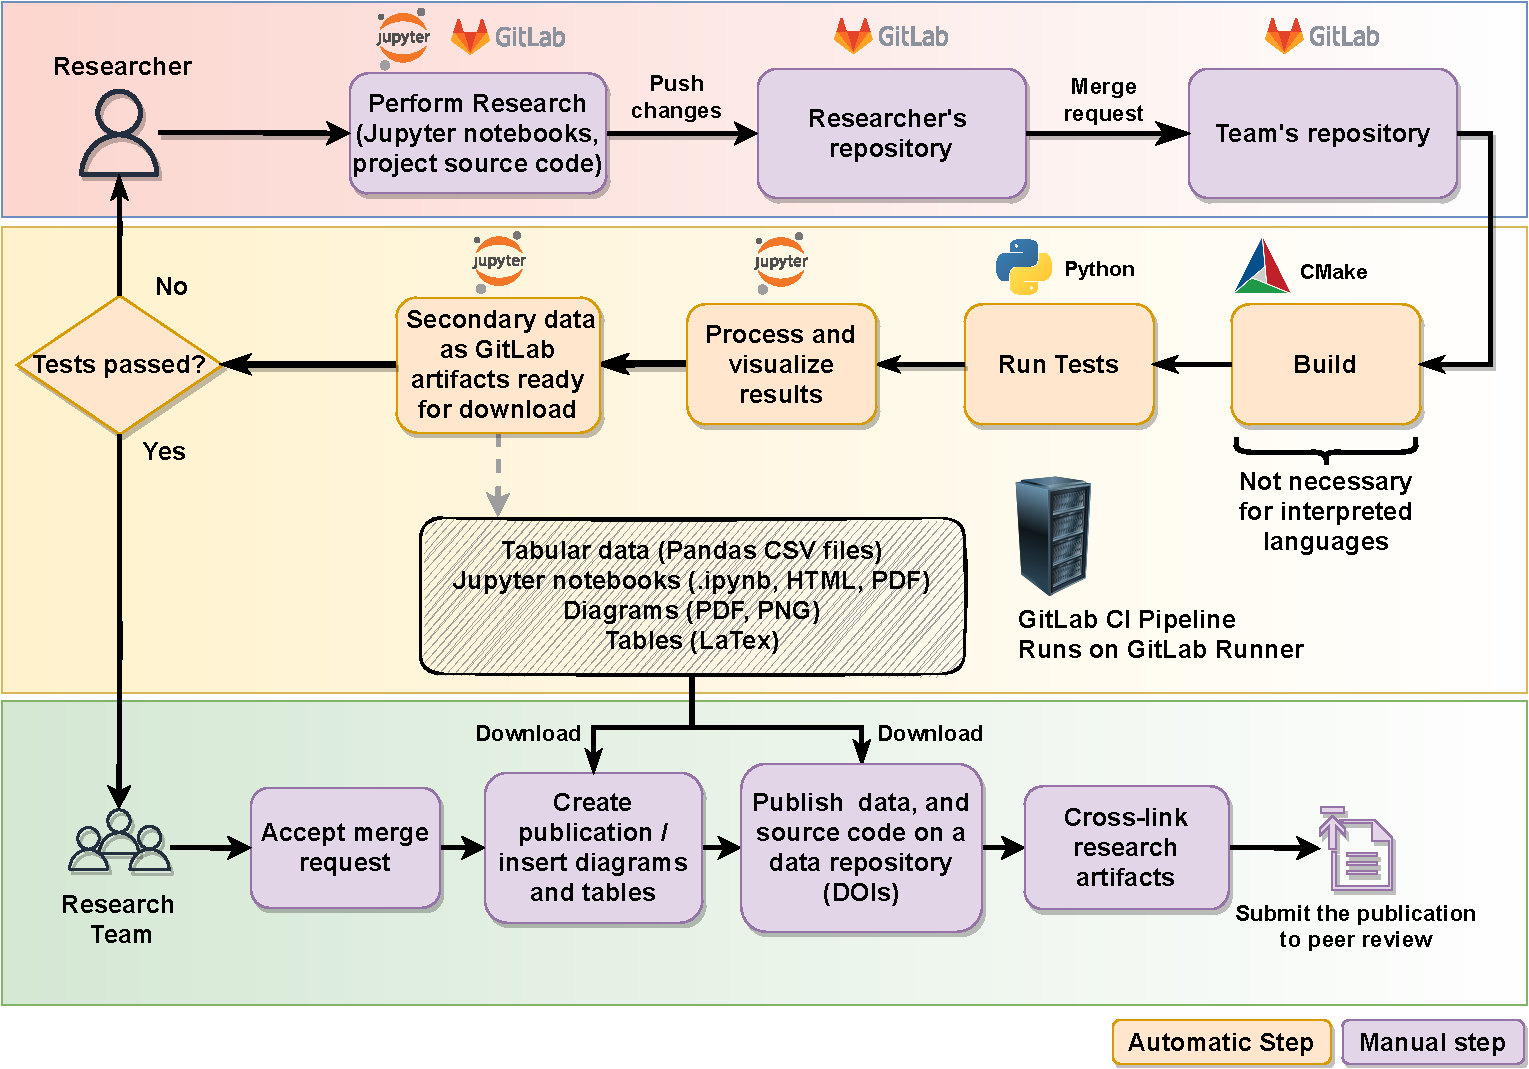
\includegraphics[width=0.8\textwidth]{figures/ZINF-CI-diagram.pdf}

\end{frame}

\begin{frame}{Continuous Integration with result visualization} 
	\framesubtitle{Parameter study organization}
	
	\begin{center}
		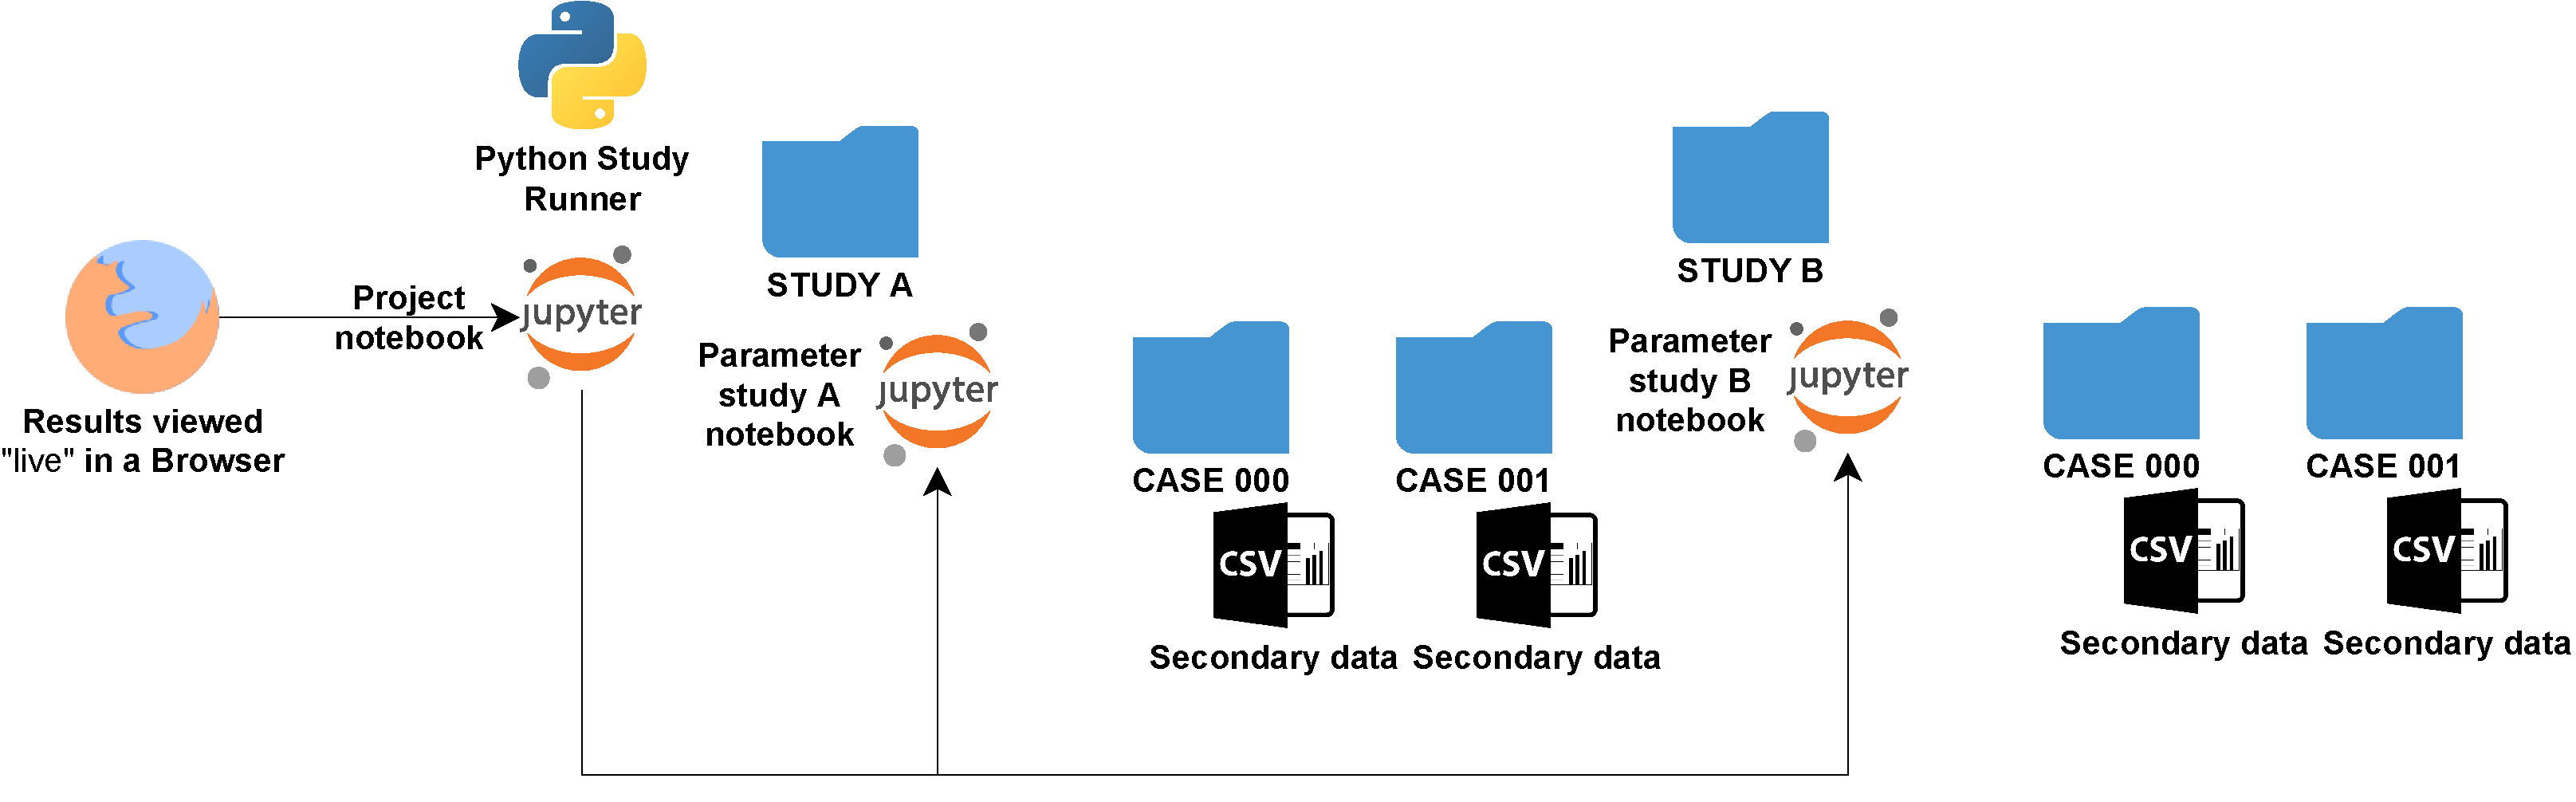
\includegraphics[width=0.8\textwidth]{figures/Cluster-Parameter-Study-Organization.pdf}
	\end{center}

	Jupyter notebooks \& python.pandas
	\begin{itemize}
		\item Doumenting the tests: geometry, input, boundary conditions, error norms, comparison data.
		\item Live visualization for long-running parameter variations. 
		\item \textbf{Simple and open format}: pandas.MultiIndex CSV files, metadata placed in columns. 
	\end{itemize}

\end{frame}

%\begin{frame}{Continuous Integration with result visualization} 
	%\framesubtitle{pandas.MultiIndex and CSV format}
	
	%\begin{itemize}
		%\item 
	%\end{itemize}

%\end{frame}

\begin{frame}{Cross-linking data, source code and reports/publications} 
	
	\vfill
	\begin{itemize}
		\item Archive secondary data on a data repository (DOI). 
		\item Archive primary data on a data repository (DOI). 
		\item Create a git tag on the remote repository. 
		\item Archive the source code, binaries and secondary data in a Singularity container (DOI). 
		\item Refer to result data DOIs, the git repo and the tag in the publication.
		\item Upload the publication to a repository (DOI, arXivID).
			\begin{itemize}
				\item For tech reports and milestones, DOIs can be requested without publication.
			\end{itemize}
		\item Edit metadata and the git-tag description until everything is cross-linked.
	\end{itemize}

\end{frame}

\begin{frame}{Cross-linking data, source code and reports/publications} 
	\framesubtitle{Schematic diagram}
	
	\begin{center}
		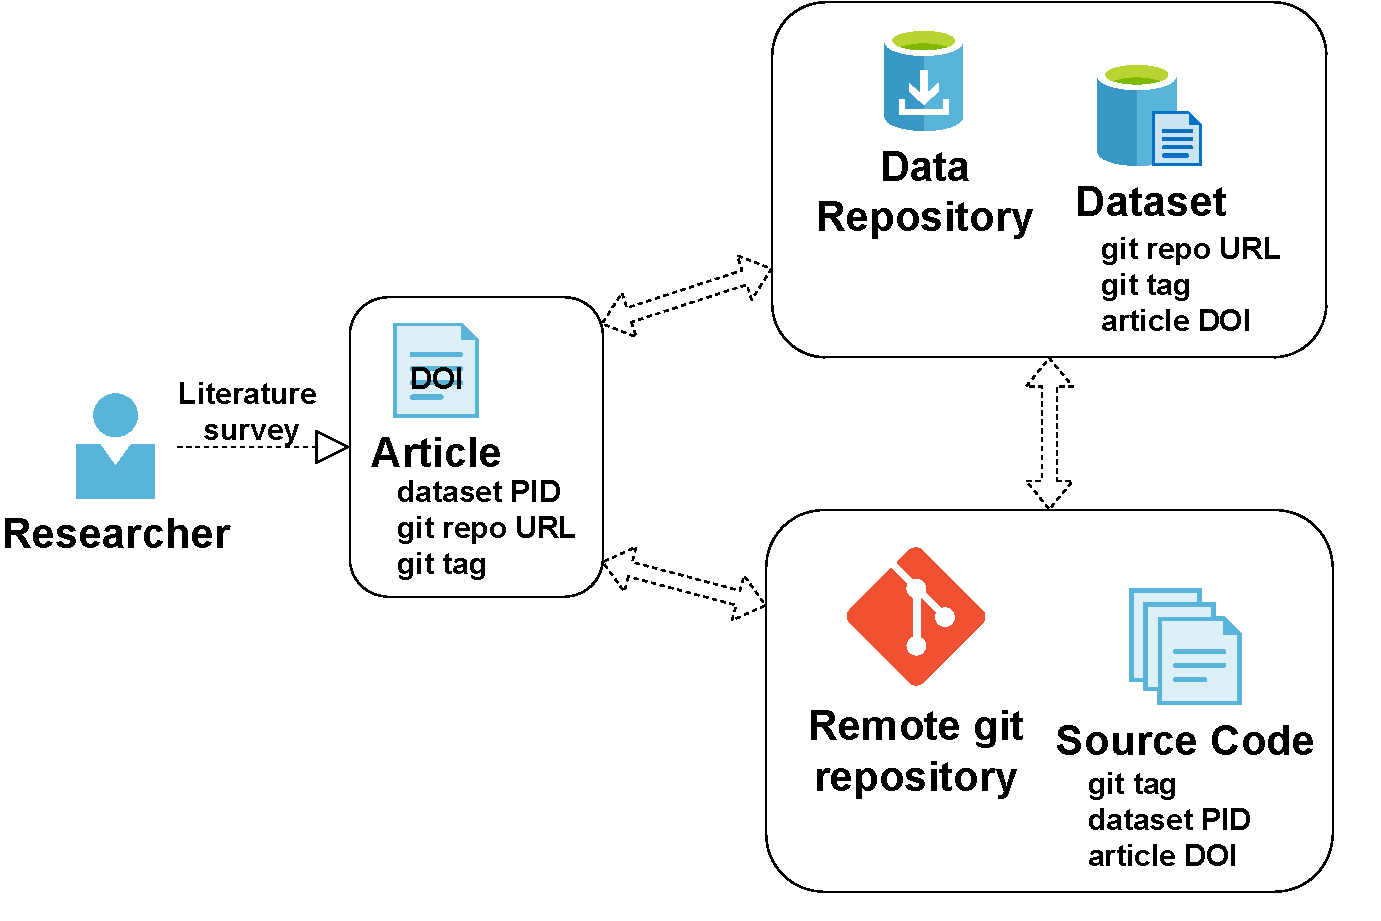
\includegraphics[width=0.6\textwidth]{figures/cross-linking.pdf}
	\end{center}

\end{frame}


\begin{frame}{Outlook}

\end{frame}

\begin{frame}{Acknowledgements}

	\vfill
	\begin{center}
		{\large 			
			Funded by the German Research Foundation (DFG) – Project-ID 265191195 – SFB 1194 : Z-INF
		}
	\end{center}

\end{frame}

\end{document}

